% % % % \input{PrivacyView}

\subsection{Privacy viewpoint}

\begin{itemize}
\item Related stakeholders: Dutch government, EU Claim
\item Related Concerns: Privacy of the user
\end{itemize}

\newpage
\begin{landscape}
\begin{figure}
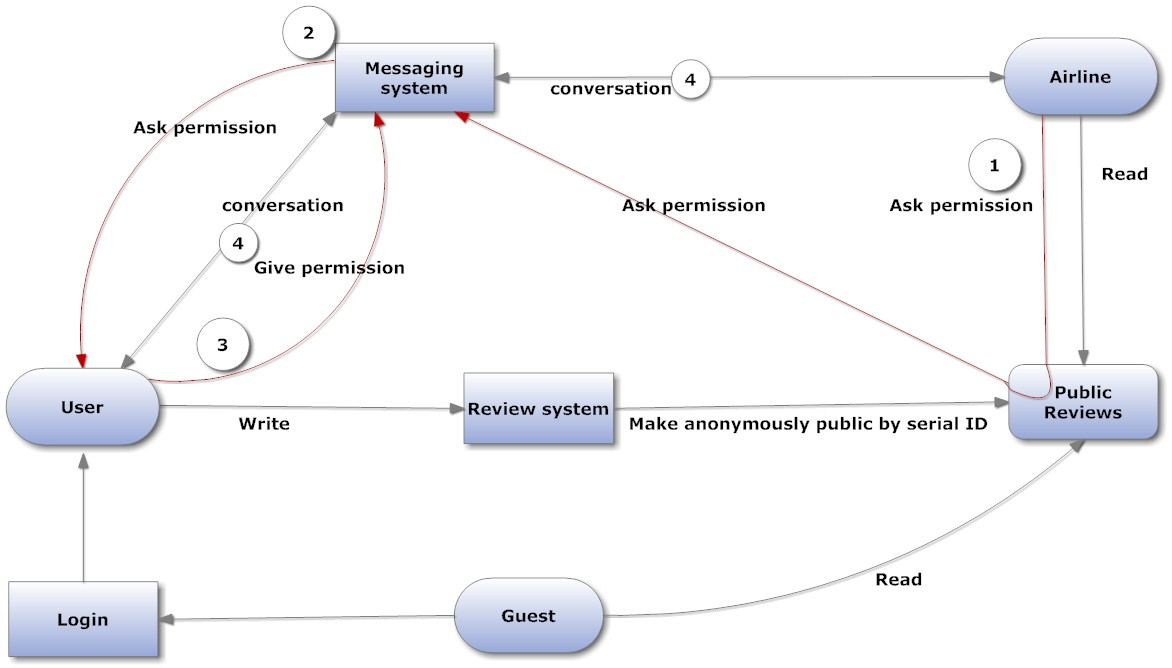
\includegraphics[width=680px]{privacyview}
\caption{Privacy viewpoint}
\label{fig:privacy}
\end{figure}
\end{landscape}
The privacy viewpoint in figure \ref{fig:privacy} shows how the privacy of the user is guaranteed in the system. A user can write a review that is shown to the public anonymously. The review will have a serialID instead of the user name so the user will stay unknown to the public. 

An airline should be able to have a conversation with an user if the airline wants to elaborate on a specific case or wants to adress the user personally. If the airline wants to get the user's information for a conversation it should ask permission of the user. When a user accepts to have a conversation with an airline the user's contact information is visible to the airline so they will be able to have a conversation. If the user is not satisfied with how the airline company responds on requests or remarks in the conversation, the user is able to invite EU Claim to the conversation so they will be able to see the conversation and decide to act upon it.

\subsection{Privacy viewpoint}

\begin{itemize}
\item Related stakeholders: Dutch government, EU Claim
\item Related Concerns: Privacy of the user
\end{itemize}

\newpage
\begin{landscape}
\begin{figure}
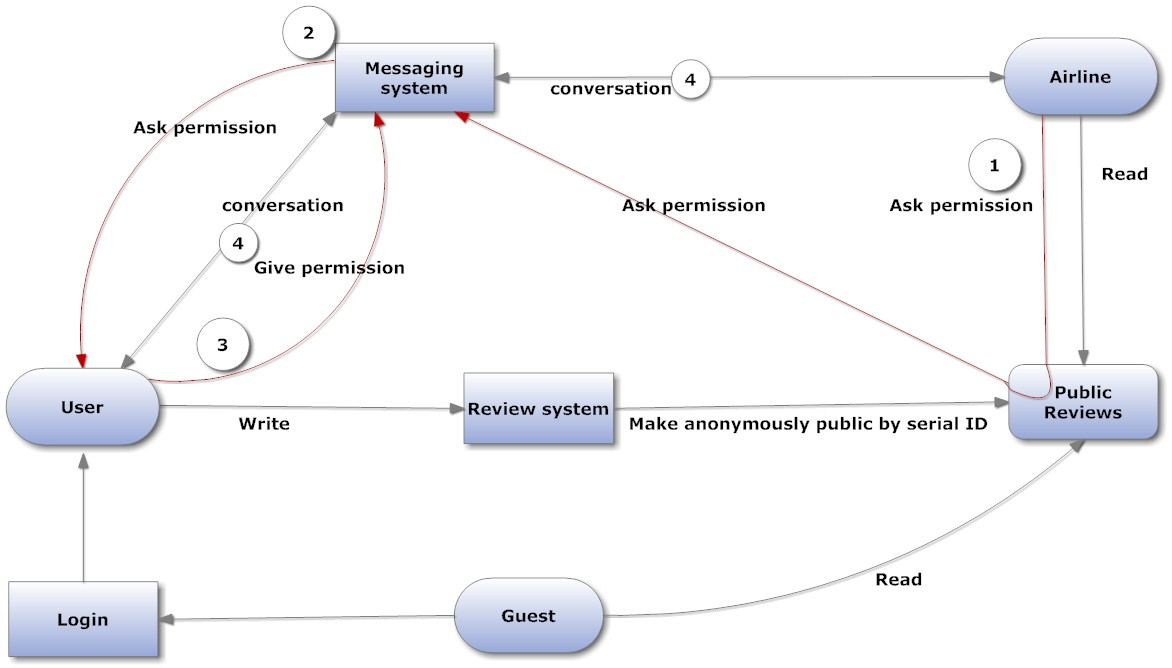
\includegraphics[width=680px]{privacyview}
\caption{Privacy viewpoint}
\label{fig:privacy}
\end{figure}
\end{landscape}
The privacy viewpoint in figure \ref{fig:privacy} shows how the privacy of the user is guaranteed in the system. A user can write a review that is shown to the public anonymously. The review will have a serialID instead of the user name so the user will stay unknown to the public. 

An airline should be able to have a conversation with an user if the airline wants to elaborate on a specific case or wants to adress the user personally. If the airline wants to get the user's information for a conversation it should ask permission of the user. When a user accepts to have a conversation with an airline the user's contact information is visible to the airline so they will be able to have a conversation. If the user is not satisfied with how the airline company responds on requests or remarks in the conversation, the user is able to invite EU Claim to the conversation so they will be able to see the conversation and decide to act upon it.

\subsection{Privacy viewpoint}

\begin{itemize}
\item Related stakeholders: Dutch government, EU Claim
\item Related Concerns: Privacy of the user
\end{itemize}

\newpage
\begin{landscape}
\begin{figure}
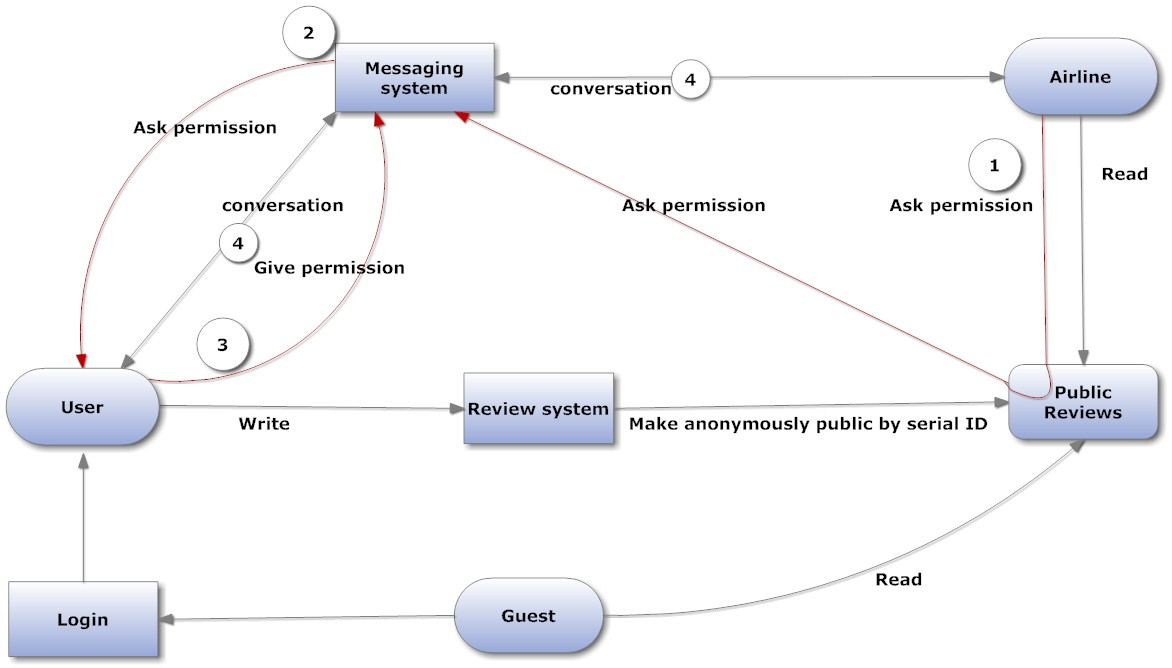
\includegraphics[width=680px]{privacyview}
\caption{Privacy viewpoint}
\label{fig:privacy}
\end{figure}
\end{landscape}
The privacy viewpoint in figure \ref{fig:privacy} shows how the privacy of the user is guaranteed in the system. A user can write a review that is shown to the public anonymously. The review will have a serialID instead of the user name so the user will stay unknown to the public. 

An airline should be able to have a conversation with an user if the airline wants to elaborate on a specific case or wants to adress the user personally. If the airline wants to get the user's information for a conversation it should ask permission of the user. When a user accepts to have a conversation with an airline the user's contact information is visible to the airline so they will be able to have a conversation. If the user is not satisfied with how the airline company responds on requests or remarks in the conversation, the user is able to invite EU Claim to the conversation so they will be able to see the conversation and decide to act upon it.

\subsection{Privacy viewpoint}

\begin{itemize}
\item Related stakeholders: Dutch government, EU Claim
\item Related Concerns: Privacy of the user
%\item Related design decisions: How will the 
\end{itemize}

\newpage
\begin{landscape}
\begin{figure}
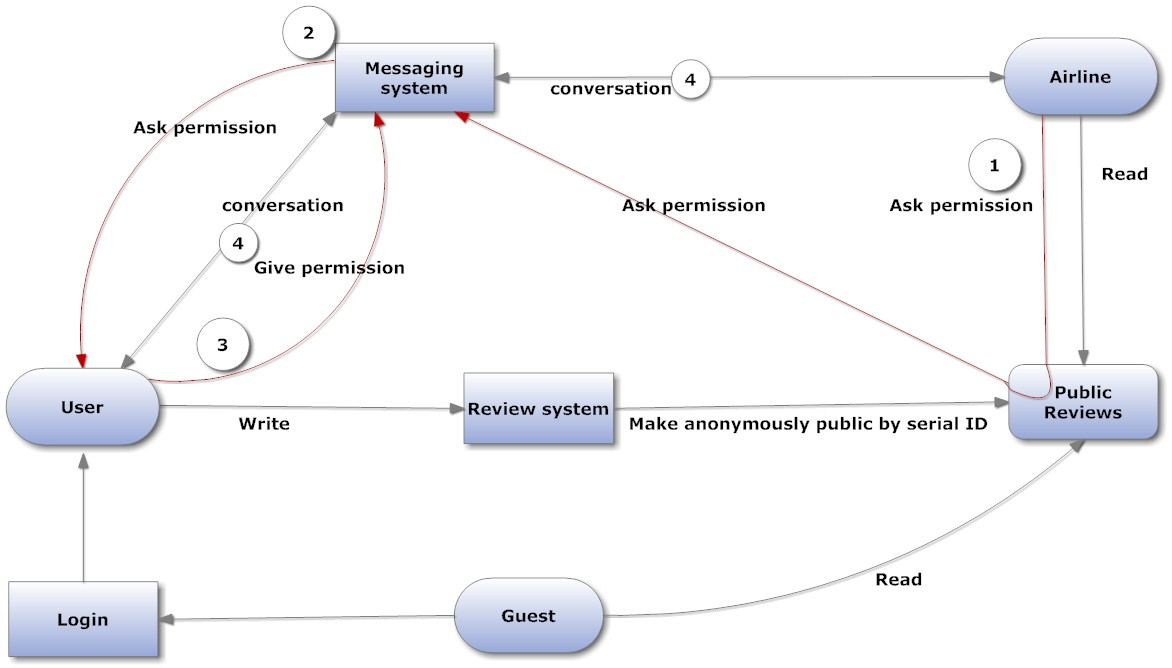
\includegraphics[width=680px]{privacyview}
\caption{Privacy viewpoint}
\label{fig:privacy}
\end{figure}
\end{landscape}

The privacy viewpoint sown in figure \ref{fig:privacy} shows how the privacy of the user is garanteed in the system. A user can write a review that is shown to the public anonymously. The review will have a serialID instead of the user name so the user will stay unknown to the public. 

An airline should be able to have a conversation with an user if the airline wants to elaborate on a specific case or wants to adress the user personally. If the airline wants to get the user's information for a conversation it should ask permission of the user. When a user accepts to have a conversation with an airline the user's contact information is visible to the airline so they will be able to have a conversation. If the user is not satisfied with how the airline company responds on requests or remarks in the conversation, the user is able to invite EU Claim to the conversation so they will be able to see the conversation and decide to act upon it.